\documentclass[border=3pt]{standalone}
% Shared preamble for all standalone figures
\usepackage[T1]{fontenc}
\usepackage{amsmath}
\usepackage{txfonts}
\usepackage{pgfplots}
\usepgfplotslibrary{groupplots,fillbetween}
\usetikzlibrary{arrows.meta,positioning,calc,shapes.misc,fit,backgrounds}
\pgfplotsset{compat=1.18}
% categorical slots (validated: adjacent CVD separation passes)
\definecolor{cA}{HTML}{2A78D6}
\definecolor{cB}{HTML}{EB6834}
\definecolor{cC}{HTML}{1BAF7A}
\definecolor{cD}{HTML}{6250D6}
% ordinal blue ramp for ordered parameter values
\definecolor{o1}{HTML}{86B6EF}
\definecolor{o2}{HTML}{3987E5}
\definecolor{o3}{HTML}{1C5CAB}
\definecolor{o4}{HTML}{0D366B}
% ink and chrome
\definecolor{ink}{HTML}{0B0B0B}
\definecolor{ink2}{HTML}{52514E}
\definecolor{ink3}{HTML}{8A8984}
\definecolor{gridc}{HTML}{E4E3DF}
\definecolor{relfill}{HTML}{E6F0FC}
\definecolor{mixfill}{HTML}{FCE9DF}
\definecolor{wfill}{HTML}{EFEEEB}
\pgfplotsset{
  paper/.style={
    width=7.55cm, height=5.2cm, scale only axis=false,
    axis lines*=left, axis line style={ink3, line width=0.4pt},
    tick style={ink3, line width=0.4pt}, tick align=outside,
    major tick length=2.5pt, minor tick length=1.5pt,
    grid=major, major grid style={gridc, line width=0.35pt},
    tick label style={font=\footnotesize, color=ink2},
    label style={font=\small, color=ink},
    title style={font=\small, color=ink, align=left, anchor=west, at={(0,1.03)}},
    every axis title shift=0pt,
    legend style={draw=none, fill=white, fill opacity=0.85, text opacity=1,
                  font=\footnotesize, text=ink2, cells={anchor=west},
                  row sep=-1pt},
    legend cell align=left,
    every axis plot/.append style={line width=1.15pt, line join=round},
    clip mode=individual,
    /pgf/number format/fixed, /pgf/number format/1000 sep={},
  },
}
\tikzset{
  lab/.style={font=\footnotesize, inner sep=1.5pt},
  vline/.style={ink3, line width=0.6pt, densely dotted},
}

\begin{document}
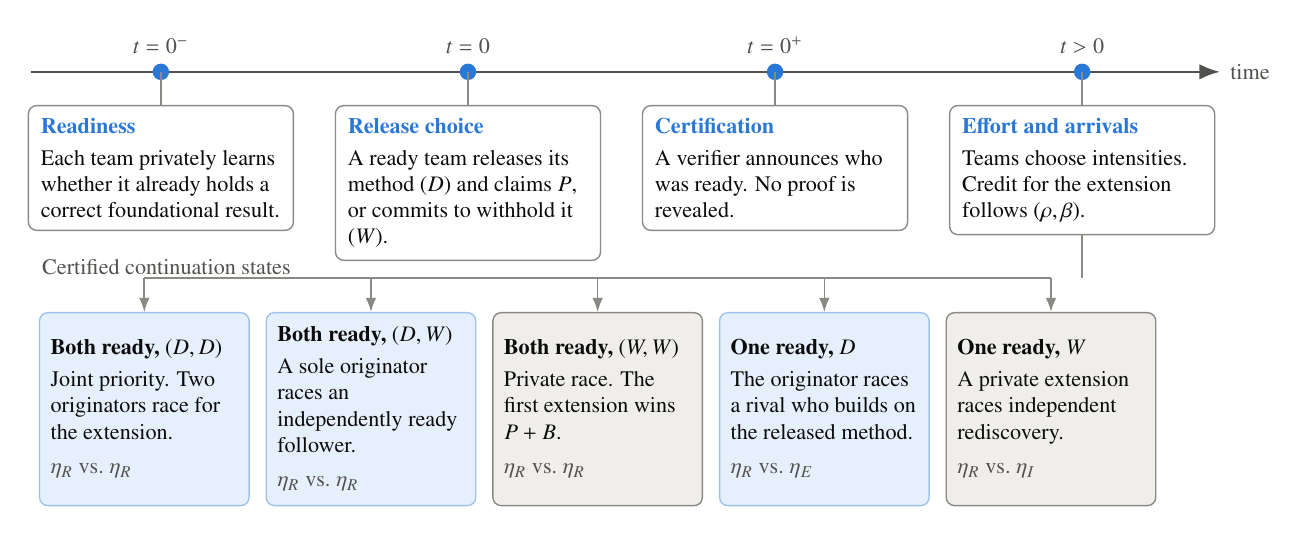
\begin{tikzpicture}[
  stage/.style={rounded corners=3pt, draw=ink3, line width=0.5pt, fill=white,
     text width=3.05cm, align=flush left, inner sep=4.5pt, font=\footnotesize, text=ink},
  state/.style={rounded corners=3pt, line width=0.5pt, text width=2.38cm,
     align=flush left, inner sep=4pt, font=\footnotesize, text=ink, minimum height=2.45cm},
  tick/.style={circle, fill=cA, inner sep=2.1pt},
]
\draw[-{Latex[length=2.6mm]}, line width=0.8pt, ink2] (-0.1,0) -- (15.0,0)
   node[right, font=\footnotesize, text=ink2] {time};
\foreach \x/\t in {1.55/{$t=0^-$}, 5.45/{$t=0$}, 9.35/{$t=0^+$}, 13.25/{$t>0$}}{
  \node[tick] at (\x,0) {};
  \node[font=\footnotesize, text=ink2, above=3pt] at (\x,0) {\t};
}
\node[stage, anchor=north] (s0) at (1.55,-0.42) {\textcolor{cA}{\textbf{Readiness}}\\[2pt]
  Each team privately learns whether it already holds a correct foundational result.};
\node[stage, anchor=north] (s1) at (5.45,-0.42) {\textcolor{cA}{\textbf{Release choice}}\\[2pt]
  A ready team releases its method ($D$) and claims $P$, or commits to withhold it ($W$).};
\node[stage, anchor=north] (s2) at (9.35,-0.42) {\textcolor{cA}{\textbf{Certification}}\\[2pt]
  A verifier announces who was ready. No proof is revealed.};
\node[stage, anchor=north] (s3) at (13.25,-0.42) {\textcolor{cA}{\textbf{Effort and arrivals}}\\[2pt]
  Teams choose intensities. Credit for the extension follows $(\rho,\beta)$.};
\foreach \x/\n in {1.55/s0, 5.45/s1, 9.35/s2, 13.25/s3}{
  \draw[ink3, line width=0.5pt] (\x,0) -- (\n.north);}
\begin{scope}[yshift=-3.05cm]
\node[state, fill=relfill, draw=cA!45, anchor=north west] (a) at (0,0) {\textbf{Both ready, $(D,D)$}\\[2pt]
  Joint priority. Two originators race for the extension.\\[3pt]\textcolor{ink2}{$\eta_R$ vs.\ $\eta_R$}};
\node[state, fill=relfill, draw=cA!45, right=0.2cm of a] (b) {\textbf{Both ready, $(D,W)$}\\[2pt]
  A sole originator races an independently ready follower.\\[3pt]\textcolor{ink2}{$\eta_R$ vs.\ $\eta_R$}};
\node[state, fill=wfill, draw=ink3, right=0.2cm of b] (c) {\textbf{Both ready, $(W,W)$}\\[2pt]
  Private race. The first extension wins $P+B$.\\[3pt]\textcolor{ink2}{$\eta_R$ vs.\ $\eta_R$}};
\node[state, fill=relfill, draw=cA!45, right=0.2cm of c] (d) {\textbf{One ready, $D$}\\[2pt]
  The originator races a rival who builds on the released method.\\[3pt]\textcolor{ink2}{$\eta_R$ vs.\ $\eta_E$}};
\node[state, fill=wfill, draw=ink3, right=0.2cm of d] (e) {\textbf{One ready, $W$}\\[2pt]
  A private extension races independent rediscovery.\\[3pt]\textcolor{ink2}{$\eta_R$ vs.\ $\eta_I$}};
\end{scope}
\coordinate (bar) at (13.25,-2.62);
\draw[ink3, line width=0.6pt] (s3.south) -- (bar);
\draw[ink3, line width=0.6pt] (a.north |- bar) -- (e.north |- bar);
\foreach \n in {a,b,c,d,e}{
  \draw[-{Latex[length=1.8mm]}, ink3, line width=0.6pt] (\n.north |- bar) -- (\n.north);}
\node[font=\footnotesize, text=ink2, anchor=south west, inner sep=1pt] at (a.north west |- bar) {Certified continuation states};
\end{tikzpicture}
\end{document}
